\documentclass{article}

%
% 引入模板的style文件
%
\usepackage{homework}

\setCJKmainfont{SimSun}[AutoFakeBold] %宋体加粗
\setCJKsansfont{SimHei}[AutoFakeBold] %黑体加粗


\usepackage{minted} %配合minted宏包进行好看的高亮
\usepackage{currfile} %配合minted宏包进行好看的高亮
\usepackage{caption} %配合minted宏包进行好看的高亮
\usepackage{tcolorbox} %配合minted宏包进行好看的高亮
\usepackage{xcolor} %配合minted宏包进行好看的高亮
\tcbuselibrary{skins} %配合minted宏包进行好看的高亮
\tcbuselibrary{minted} %配合minted宏包进行好看的高亮
\usemintedstyle{paraiso-dark} %配合minted宏包进行好看的高亮
\usepackage{framed} 


%
% 封面
%


\title{
	
\includegraphics[width=0.5\textwidth]{images/title/ucas_logo 1.pdf}\\
    \vspace{1in}
    \textmd{\textbf{\hmwkClass}}\\
	\textmd{\Large{\textbf{\hmwkClassID}}}\\
    \textmd{\textbf{\hmwkTitle}}\\
    \normalsize\vspace{0.1in}\large{\hmwkCompleteTime }\\
    \vspace{0.1in}\large{\textit{\hmwkClassInstructor\ }}\\
    \vspace{1in}
	
\includegraphics[width=0.25\textwidth]{images/title/Cyber.jpg}\\
	\vspace{1in}
}

\author{
	\hmwkAuthorName \\ 
	\hmwkAuthorStuID \\
	\hmwkAuthorInst \\
	\hmwkAuthorzhuanye \\
	\hmwkAuthorfangxiang
	}
\date{}

\renewcommand{\part}[1]{\textbf{\large Part \Alph{partCounter}}\stepcounter{partCounter}\\}


%
% 正文部分
%
\begin{document}


\maketitle


%\include{chapters/ch01}
%\include{chapters/ch02}
%\include{chapters/ch03}
%\include{chapters/ch04}
%\include{chapters/ch05}


\begin{homeworkProblem}
	\textbf{打家劫舍}: 一个强盗正计划抢劫沿街的房子. 每间房子都藏有一定数量的钱, 阻止你抢劫每间房子的唯一限制是相邻的房子都连接了安全系统, 如果两间相邻的房子在同一晚被闯入, 它会自动联系警方.

	1. 给出一个非负整数列表, 表示每所房子的金额, 确定你今晚可以在不报警的情况下抢劫的最大金额;

	2. 如果所有的房子都排成一个圈呢?
	\\

	\solution \,\,1. \textbf{算法思想}: 对于第$i$个房间, 如果决定抢劫, 那么第$i-1$间房就不能抢, 即所抢到的金额就是前$i-2$间房间所抢到的钱再加上$a[i]$; 若不抢劫第$i$间房子, 那么所抢到的金额就是前$i-1$间房间所抢到的钱.
	
	\textbf{最优子结构}: 设$\text{dp}[i]$表示前$i$间房屋能偷窃到的最高总金额, 假设$\left[ a_{m_1},a_{m_2},\cdots ,a_{m_k} \right] $为(前$i$间房子中)所抢的房间列表, 那么$\left[ a_{m_1},a_{m_2},\cdots ,a_{m_{k-1}} \right]$一定是(前$i-1$间房子中)所抢的房间列表. 否则, 若$\left[ a_{t_1},a_{t_2},\cdots ,a_{t_{k-1}} \right]$是(前$i-1$间房子中)所抢的房间列表\footnote{显然前$i-1$间房子中必须抢$k-1$间房子, 否则如果更少的话(比如$k-2$), 那么考虑前$i$个房子的抢劫时, 数量就对不上$k$个了.}, 则$\left[ a_{t_1},a_{t_2},\cdots ,a_{t_{k-1}},a_{m_k} \right] $一定是前$i$间房子中所抢的列表. 即与$\left[ a_{m_1},a_{m_2},\cdots ,a_{m_{k-1}},a_{m_k} \right] $是前$i$间房子中所抢的列表相矛盾, 即这样定义的子问题具有\textbf{递归性}(即满足最优子结构). 根据上述的算法思想可以写出如下递推表达式:
	$$
	dp\left[ i \right] =\text{max} \left\{ dp\left[ i-2 \right] +a\left[ i \right] ,dp\left[ i-1 \right] \right\} , \,\,  2\le i\le n-1
	$$
	当只有一间房子时, 则$dp[0]=a[0]$; 若只有两间房子, 则$dp[1]=\text{max}\left\{ a[0], a[1] \right\}$. 于是可以写出如下C++代码(已完全通过\href{https://leetcode.cn/problems/house-robber/description/}{\textbf{LeetCode-T198}}的所有测试样例.):
\begin{tcblisting}{listing engine=minted,boxrule=0.1mm,
colback=blue!5!white,colframe=blue!75!black,
listing only,left=5mm,enhanced,sharp corners=all,
overlay={\begin{tcbclipinterior}\fill[red!20!blue!20!white] (frame.south west)
rectangle ([xshift=5mm]frame.north west);\end{tcbclipinterior}},
minted language=c++,
minted style=tango,
minted options={fontsize=\small,breaklines,autogobble,linenos,numbersep=3mm}}
class Solution {
public:
    int rob(vector<int>& nums) {
        int n = nums.size();
        if(n == 1) {
            return nums[0];
        }
        else if(n == 2) {
            return max(nums[0],nums[1]);
        }
        else {
            vector<int> dp(n, 0);
            dp[0] = nums[0];
            dp[1] = max(nums[0],nums[1]);
            for(int i = 2; i <= n - 1; i++) {
                dp[i] = max(dp[i - 2] + nums[i], dp[i - 1]);
            }
            return dp[n - 1];
        }
    }
};
\end{tcblisting}
	\newpage
	2. 如果是环形数组的情形, 那么可以如下考虑. \textbf{算法思想}: 如果第1个房间打劫了, 那么最后一个房间就不能打劫了; 如果第1个房间没被打劫, 那么最后一个房间就可以打劫. 这两种情形分别按照上述方法求出最高金额, 再取最大值即可. 于是我们可以写出两种情况下分别对应的递推表达式:
	\begin{align}
		dp_1\left[ i \right] &=\text{max} \left\{ dp_1\left[ i-2 \right] +a\left[ i \right] ,dp_1\left[ i-1 \right] \right\} ,  2\le i\le n-2 \notag
		\\
		dp_2\left[ i \right] &=\text{max} \left\{ dp_2\left[ i-2 \right] +a\left[ i \right] ,dp_2\left[ i-1 \right] \right\} ,  2\le i\le n-1 \notag
	\end{align}
	以及对应的边界条件
	$$
	dp_1\left[ 0 \right] =a\left[ 0 \right] , dp_1\left[ 1 \right] =\text{max} \left\{ a\left[ 0 \right] ,a\left[ 1 \right] \right\} ;\,\, dp_2\left[ 0 \right] =0, dp_2\left[ 1 \right] =a\left[ 1 \right] 
	$$
	最后返回$$\text{res}=\text{max} \left\{ dp_1\left[ n-2 \right] ,dp_2\left[ n-1 \right] \right\} $$
	算法具体的C++代码如下(已完全通过\href{https://leetcode.cn/problems/house-robber-ii/description/}{\textbf{LeetCode-T213}}的所有测试样例.). 两个算法的时空复杂度显然都是$O(n)$.
\begin{tcblisting}{listing engine=minted,boxrule=0.1mm,
colback=blue!5!white,colframe=blue!75!black,
listing only,left=5mm,enhanced,sharp corners=all,
overlay={\begin{tcbclipinterior}\fill[red!20!blue!20!white] (frame.south west)
rectangle ([xshift=5mm]frame.north west);\end{tcbclipinterior}},
minted language=c++,
minted style=tango,
minted options={fontsize=\small,breaklines,autogobble,linenos,numbersep=3mm}}
class Solution {
public:
    int rob(vector<int>& nums) {
        int n = nums.size();
        if(n == 1) {
            return nums[0];
        }
        else if(n == 2) {
            return max(nums[0], nums[1]);
        }
        else {
            vector<int> dp1(n, 0); //第1个房间抢劫
            vector<int> dp2(n, 0); //第1个房间不抢劫
            dp1[0] = nums[0];
            dp1[1] = max(nums[0], nums[1]);
            for(int i = 2; i <= n - 2; i++) {
                dp1[i] = max(dp1[i - 2] + nums[i], dp1[i - 1]);
            }
            dp2[0] = 0;
            dp2[1] = nums[1];
            for(int i = 2; i <= n - 1; i++) {
                dp2[i] = max(dp2[i - 2] + nums[i], dp2[i - 1]);
            }
            int res = max(dp1[n - 2], dp2[n - 1]);
            return res;
        }
    }
};
\end{tcblisting}
\end{homeworkProblem}


\pagebreak

\begin{homeworkProblem}
	\textbf{丑数}: 一个正整数的素因子仅局限于2,3,5时, 那么这个数被称作丑数. 给定一个整数$n$, 返回第$n$个丑数.

	\solution \textbf{方法1 (数学+一次遍历)}: 先运行特定算法来检验任意一个正整数是否是丑数, 然后从1到$+\infty$开始检验每一个正整数(for循环)并维护一个变量cnt, 如果是丑数, 那么cnt++, 如果cnt==$n$, 那么退出for循环并返回当前数. 
	
	\textbf{判断是否是丑数的逻辑}: 若$n$是丑数, 即$n$会形如$n=2^a\cdot 3^b\cdot 5^c$. 于是先拿2不断的去除$n$, 除到(模2的)余数不为零为止; 在除完$2^a$之后, 再拿3不断的去除$n$, 除到(模3的)余数不为零为止; 在除完$3^b$之后, 再拿5不断的去除$n$, 除到(模5的)余数不为零为止. 如果此时$n=1$那么$n$是丑数, 否则不是丑数. 算法的C++代码见如下:
\begin{tcblisting}{listing engine=minted,boxrule=0.1mm,
colback=blue!5!white,colframe=blue!75!black,
listing only,left=5mm,enhanced,sharp corners=all,
overlay={\begin{tcbclipinterior}\fill[red!20!blue!20!white] (frame.south west)
rectangle ([xshift=5mm]frame.north west);\end{tcbclipinterior}},
minted language=c++,
minted style=tango,
minted options={fontsize=\small,breaklines,autogobble,linenos,numbersep=3mm}}
class Solution {
public:
    int nthUglyNumber(int n) {
        int cnt = 0;
        int i = 1;
        for(; cnt != n; i++) {
            if(isUgly(i) == true) {
                cnt++;
            }
        }
        return i - 1;
    }
    bool isUgly(int n) {
        if(n <= 0) {
            return false;
        }
        else {
            vector<int> factors = {2, 3, 5};
            for(int factor : factors) {
                while(n % factor == 0) {
                    n /= factor;
                }
            }
            return n == 1;
        }
    }
};
\end{tcblisting}
	该算法(的数学逻辑)显然是正确的, 就不用单独证明了. 经过实验, 该算法在LeetCode平台上执行起来是超时的. 算法超时只要是因为丑数的分布过于稀疏, 从而导致大量非丑数的判别. 并且可知, 当$n$很大时, 第$n$个丑数的值是$n$的指数级, 也就是说, for循环需要指数次(不妨记作$M^n$, 其中$M>1$). 而判断一个数$i$是否为丑数需要$O(\log i)$的时间, 于是可以推出整个算法的时间复杂度为$$T\left( n \right) =\sum_{i=1}^{M^n}{\log i}=\log \left( 1\cdot 2\cdot 3\cdots M^n \right) =\log \left\{ \left( M^n \right) ! \right\} =O\left( n\cdot M^n \right) 
	$$
	注意, 根据斯特林公式可知: $$n!\sim \sqrt{2\pi n}\left( \frac{n}{e} \right) ^n\Rightarrow \left( M^n \right) !\sim \sqrt{2\pi M^n}\left( \frac{M^n}{e} \right) ^{M^n}\Rightarrow \log \left\{ \left( M^n \right) ! \right\} \sim n\cdot M^n
	$$
	\newpage
	\textbf{方法2 (三指针动态规划)}: 定义数组$dp$, 其中$dp[i]$表示第$i$个丑数, 则答案为$dp[n]$. 易知, 最小的丑数为1, 即$dp[1]=1$. 这里我们需要定义三个指针$p^{(2)},p^{(3)},p^{(5)}$, 指针$p^{(x)}(x\in \{2,3,5\})$的含义是: 使得$dp[j]\times x>dp[i-1]$的最小下标$j$(注意$1\leq j\leq i-2$). 那么计算下一个丑数$dp[i]$, 会出现三种可能情况: 
	
	\textbf{1.} 通过前面一堆丑数$d[1,\cdots,i-1]$中的\textbf{某一个丑数}乘以2得到的:
	
	举个例子, 一串丑数1,2,3,4,5,6,8,9,10,12, 其中$1\times 2,2\times 2, 3\times 2, 4\times 2, 5\times 2, 6 \times 2$\textbf{已经出现过了}! 故所谓的"某一个丑数"就是指针$p^{(2)}$所指向的元素8, 即这种情形(\textbf{决策})下, 下一个丑数就是$dp\left[ p^{\left( 2 \right)} \right] \times 2$; 
	
	\textbf{2.} 通过前面一堆丑数$d[1,\cdots,i-1]$中的\textbf{某一个丑数}乘以3得到的:
	
	举个例子, 一串丑数1,2,3,4,5,6,8,9,10,12, 其中$1\times 3,2\times 3, 3\times 3, 4\times 3$\textbf{已经出现过了}! 故所谓的"某一个丑数"就是指针$p^{(3)}$所指向的元素5, 即这种情形(\textbf{决策})下, 下一个丑数就是$dp\left[ p^{\left( 3 \right)} \right] \times 3$;

	\textbf{3.} 通过前面一堆丑数$d[1,\cdots,i-1]$中的\textbf{某一个丑数}乘以5得到的:

	举个例子, 一串丑数1,2,3,4,5,6,8,9,10,12, 其中$1\times 5,2\times 5$\textbf{已经出现过了}! 故所谓的"某一个丑数"就是指针$p^{(5)}$所指向的元素3, 即这种情形(\textbf{决策})下, 下一个丑数就是$dp\left[ p^{\left( 5 \right)} \right] \times 5$.

	因此, 计算$dp[i]$时只需要在上述三种可能决策对应的结果中取一个最小值就行了(否则就跨过某个丑数了), 如果$dp[i]$来源于乘$x(\in \left\{ 2,3,5 \right\})$得到的, 那么指针$p^{(x)}$需要往前移一位(否则, 如果$dp[i+1]$还来源于乘以$x$得到的话, 就会出现计算重复). 

	\textbf{正确性证明}: 注意到指针$p^{(x)}$的定义, 可知当$1\leq j\leq p^{(x)}-1$时, $dp[j]\times x\leq dp[i-1]$. 所以令(即递推表达式)
	$$
	dp\left[ i \right] =\text{min} \left\{ dp\left[ p^{\left( 2 \right)} \right] \times 2,dp\left[ p^{\left( 3 \right)} \right] \times 3,dp\left[ p^{\left( 5 \right)} \right] \times 5 \right\} ,2\le i\le n
	$$
	即可使得$dp[i]>dp[i-1]$且$dp[i]$是大于$dp[i-1]$的最小丑数. 算法的C++代码如下所示, 已完全通过\href{https://leetcode.cn/problems/ugly-number-ii/description/}{\textbf{LeetCode-T264}}的所有测试样例.
\begin{tcblisting}{listing engine=minted,boxrule=0.1mm,
colback=blue!5!white,colframe=blue!75!black,
listing only,left=5mm,enhanced,sharp corners=all,
overlay={\begin{tcbclipinterior}\fill[red!20!blue!20!white] (frame.south west)
rectangle ([xshift=5mm]frame.north west);\end{tcbclipinterior}},
minted language=c++,
minted style=tango,
minted options={fontsize=\small,breaklines,autogobble,linenos,numbersep=3mm}}
class Solution {
public:
    int nthUglyNumber(int n) {
        vector<int> dp(n + 1, 0);
        dp[1] = 1;
        int p2 = 1, p3 = 1, p5 = 1;  //三指针的初始化
        for(int i = 2; i <= n; i++) {
            int num2 = dp[p2] * 2, num3 = dp[p3] * 3, num5 = dp[p5] * 5;
            dp[i] = min(num2, min(num3, num5));
            if(dp[i] == num2) {
                p2++;
            }
            if(dp[i] == num3) {
                p3++;
            }
            if(dp[i] == num5) {
                p5++;
            }
        }
        return dp[n];
    }
};
\end{tcblisting}
	显然, 该算法的时间复杂度为$O(n)$, 空间复杂度也为$O(n)$.
\end{homeworkProblem}

\pagebreak


\begin{homeworkProblem}
	给定一组互异的正整数集合, 找到最大子集: 使得子集元素中的每一对$(S_i,S_j)$都满足$S_i\%S_j=0$或$S_j\% S_i=0$. 请返回最大子集的阶数(即子集中的元素个数). \textbf{注意}: $S_i\%S_j=0$意味着$S_i$可以被$S_j$整除.

	\solution 在解决这个问题之前, 我们需要先给出另一个解决思路与此非常类似的问题以便进行类比学习: \textbf{最长单增子序列问题}. 问题是说, 给定一个元素彼此互异的整型数组, 请你给出该数组的最长单调递增子序列(及其长度). 
    
    定义$dp[i]$是以$\text{nums}[i]$\textbf{为结尾}(且考虑前$i$个元素)的最长单增子序列的长度. 
    \begin{itemize}
        \item 如果在索引范围$[0,i-1]$当中能够找到(若干个)下标$j$使得$\text{nums}[j]<\text{nums}[i]$成立. 根据\textbf{大小关系的传递性}可知: 以$\text{nums}[j]$为结尾的最长递增子序列中的所有元素都$<\text{nums}[i]$, 也就是说我们找到了符合条件的位置. 那么在这些位置$j$中找到$dp[j]$的最大值, 在此基础上加1即可使得以$\text{nums}[i]$为结尾的单增子序列长度最大(即将nums$[i]$接到符合条件的、且最长的nums$[j]$后边).
        \item 如果在索引范围$[0,i-1]$当中找不到下标$j$使得$\text{nums}[j]<\text{nums}[i]$成立(即$\text{nums}[0,\cdots,i-1]$都比$\text{nums}[i]$大), 那么以nums$[i]$为结尾的单增子序列长度就只能为1(即nums$[i]$独立作为单增子序列).
    \end{itemize}

    故综合上述两种情况, 我们可以写出如下转移方程$(i\geq 1)$和初始条件:
    $$
    dp\left[ i \right] =\left\{ \begin{matrix}
        \underset{0\le j\le i-1}{\text{max}}dp\left[ j \right] +1,&		\exists j\in \left[ 0,i-1 \right] , s.t. \,\text{nums}\left[ j \right] <\text{nums}\left[ i \right]\\
        1&		\forall j\in \left[ 0,i-1 \right] , s.t. \,\text{nums}\left[ j \right] >\text{nums}\left[ i \right]\\
    \end{matrix} \right. , dp\left[ 0 \right] =1
    $$

    但是上述递推方程只能给出长度, 并不能给出具体的最优解, 所以我们需要借助一个数组$m$来对解进行回溯\footnote{对于求\textbf{具体方案}的动态规划题目, 多开一个数组来记录状态的转移情况是\textbf{最常见}的手段.}(即$m[i]$记录$dp[i]$是由哪个下标的状态转移而来的). 而要想算出\textbf{整个数组}的最长单增子序列长度, 则需要算好所有的$dp[i]$值, 再对$dp$数组进行遍历, 由此得到最长单增子序列长度和对应下标\footnote{因为整个数组的最长单增子序列\textbf{不一定}以nums$[n-1]$为结尾! 故才需要求得$dp$数组的最大值.}. 最后使用数组$m$进行回溯以取得答案.

    类似的, 我们再来解决本题: 由于整除子集中的每一对值都是倍数\textbf{或}约数关系, 因此为了后续解决问题的方便, 我们不妨先将数组nums进行排序(耗时为$O(n\log n)$, (后续可知)不影响整个算法的复杂度), 以免还要具体考虑一对值\textbf{到底是}倍数关系还是约数关系(思考起来会很乱), 并且对nums排好序有助于我们利用\textbf{整除关系的传递性}来进行动态规划! 
    
    于是我们定义: $dp[i]$是以$\text{nums}[i]$\textbf{为结尾}(且考虑前$i$个元素)的最大整除子集的阶数(即该子集合的元素个数).
    \begin{itemize}
        \item 如果在索引范围$[0,i-1]$当中能够找到(若干个)下标$j$使得$\text{nums}[i] \% \text{nums}[j]\text{==}0$成立. 由于$\text{nums}[j]\,|\,\text{nums}[i]$且根据\textbf{整除关系的传递性}可知: 以$\text{nums}[j]$为结尾的最大整除子集中的所有元素都能整除$\text{nums}[i]$, 也就是说我们找到了符合条件的位置. 那么在这些位置$j$中找到$dp[j]$的最大值, 在此基础上加1即可使得以$\text{nums}[i]$为结尾的整除子集的长度最大(即将nums$[i]$接到符合条件的、且最长的nums$[j]$后边).
        \item 如果在索引范围$[0,i-1]$当中找不到下标$j$使得$\text{nums}[i] \% \text{nums}[j]\neq 0$成立(即$\text{nums}[i]$不能接在位置$i$之前的任何数的后面!), 那么以nums$[i]$为结尾的最大整除子集的长度就只能为1(即nums$[i]$独立作为最大整除子集).
    \end{itemize}
    故综合上述两种情况, 我们可以写出如下转移方程$(i\geq 1)$和初始条件:
    $$
    dp\left[ i \right] =\left\{ \begin{matrix}
        \underset{0\le j\le i-1}{\text{max}}dp\left[ j \right] +1,&		\exists j\in \left[ 0,i-1 \right] , s.t.\, \text{nums}\left[ i \right] \%\text{nums}\left[ j \right] =0\\
        1&		\forall j\in \left[ 0,i-1 \right] , s.t. \,\text{nums}\left[ i \right] \%\text{nums}\left[ j \right] \ne 0\\
    \end{matrix} \right. , dp\left[ 0 \right] =1
    $$
    此时我们需要借助一个数组$m$来对解进行回溯(即$m[i]$记录$dp[i]$是由哪个下标的状态转移而来的). 而要想算出\textbf{整个数组}的整除子集的最大长度, 则需要算好所有的$dp[i]$值, 再对$dp$数组进行遍历, 由此得到最大的整除子集长度和对应下标. 最后使用数组$m$进行回溯以取得答案. 于是我们可以给出最大整除子集算法的C++代码:
\begin{tcblisting}{listing engine=minted,boxrule=0.1mm,
colback=blue!5!white,colframe=blue!75!black,
listing only,left=5mm,enhanced,sharp corners=all,
overlay={\begin{tcbclipinterior}\fill[red!20!blue!20!white] (frame.south west)
rectangle ([xshift=5mm]frame.north west);\end{tcbclipinterior}},
minted language=c++,
minted style=tango,
minted options={fontsize=\small,breaklines,autogobble,linenos,numbersep=3mm}}
class Solution {
public:
    vector<int> largestDivisibleSubset(vector<int>& nums) {
        sort(nums.begin(), nums.end());  //先对数组进行排序, 方便后续考虑递推表达式
        int n = nums.size();
        vector<int> dp(n, 0);
        dp[0] = 1;
        vector<int> m(n, 0); // m[0] = 0
        for (int i = 1; i <= n - 1; i++) {
            int prev = i, len = 1; //至少包含自身一个数, 因此起始长度为1, 由自身转移而来
            for (int j = 0; j <= i - 1; j++) {
                if (nums[i] % nums[j] == 0) {  //找到满足条件的位置j
                    if (dp[j] + 1 > len) {
                        len = dp[j] + 1;
                        prev = j; //迭代式更新求得满足条件的d[j]+1的最大值和dp[i]的来源(即prev)
                    }
                }
            }
            dp[i] = len, m[i] = prev; // m[i]就是nums[i]的来源位置(即prev)!
        }
        int index = max_element(dp.begin(), dp.end()) - dp.begin(); //最大值对应的索引
        int MaxLen = dp[index]; //整除子集的最大长度值
        vector<int> res; //注意整个数组的最大整除子集是以nums[index]为结尾的!
        while (res.size() != MaxLen) {
            res.push_back(nums[index]);
            index = m[index]; //逐步地从后往前回溯索引, 并将对应元素写进res数组
        }
        reverse(res.begin(), res.end()); //reverse一下更好看一些, 此步可以选择注释掉
        return res;
    }
};
\end{tcblisting}
    上述C++代码已完全通过\href{https://leetcode.cn/problems/largest-divisible-subset/description/}{\textbf{LeetCode-T368}}的所有测试样例. 再来分析一下该算法的时空复杂度: 排序需要$O(n\log n)$的时间, 算法主体显然需要消耗$O(n^2)$的时间, 而其余操作(如reverse操作、求dp最大值以及结果写入)均只需要$O(n)$的时间, 所以综合可得算法的时间复杂度为$O(n^2)$. 由于借助了两个长度为$n$的中间数组, 所以算法的空间复杂度为$O(n)$. 类似地, 最长递增子序列问题的算法也是需要$O(n^2)$的时间和$O(n)$的空间, 算法的C++代码如后页所示, 并且已完全通过\href{https://leetcode.cn/problems/longest-increasing-subsequence/description/}{\textbf{LeetCode-T300}}的所有测试样例. 上述两个算法之所以正确, 本质上是利用了\textbf{二元关系的可传递性}. 比如最长递增子序列是利用了\textbf{大小关系“$>$”的可传递性}, 而最大整除子集利用了\textbf{整除关系“$\mid$”的可传递性}. 所以老师要是考试出类似的作业题的话, 很有可能采用其他具有\textbf{可传递性}的二元关系来出题, 请读者务必注意!(而且这两段代码基本一样, 所以可以将此记住作为解题模板, 以便应付其他具有传递性的二元关系的dp算法题)

    \newpage
\begin{tcblisting}{listing engine=minted,boxrule=0.1mm,
colback=blue!5!white,colframe=blue!75!black,
listing only,left=5mm,enhanced,sharp corners=all,
overlay={\begin{tcbclipinterior}\fill[red!20!blue!20!white] (frame.south west)
rectangle ([xshift=5mm]frame.north west);\end{tcbclipinterior}},
minted language=c++,
minted style=tango,
minted options={fontsize=\small,breaklines,autogobble,linenos,numbersep=3mm}}
#include <algorithm>
#include <ctime>
#include <iostream>
#include <vector>
using namespace std;
vector<int> LIS(vector<int>& nums) {
    int n = nums.size();
    vector<int> dp(n, 0);
    dp[0] = 1;
    vector<int> m(n, 0); // m[0] = 0
    for (int i = 1; i <= n - 1; i++) {
        int prev = i, len = 1; //至少包含自身一个数, 因此起始长度为1, 由自身转移而来
        for (int j = 0; j <= i - 1; j++) {
            if (nums[j] < nums[i]) { //找到满足条件的位置j
                if (dp[j] + 1 > len) {
                    len = dp[j] + 1;
                    prev = j; //迭代式更新求得满足条件的d[j]+1的最大值和dp[i]的来源(即prev)
                }
            }
        }
        dp[i] = len, m[i] = prev; // m[i]就是nums[i]的来源位置(即prev)!
    }
    int index = max_element(dp.begin(), dp.end()) - dp.begin(); //最大值对应的索引
    int MaxLen = dp[index]; //递增子序列的最大长度值
    vector<int> res; //注意整个数组的最长递增子序列是以nums[index]为结尾的!
    while (res.size() != MaxLen) {
        res.push_back(nums[index]);
        index = m[index]; //逐步地从后往前回溯索引, 并将对应元素写进res数组
    }
    reverse(res.begin(), res.end()); //reverse一下更好看一些, 此步可以选择注释掉
    return res;
}
int main() {
    int n;
    cin >> n;            //输入数组的长度
    vector<int> nums(n); //定义数组
    cout << "数组nums为:" << endl;
    for (int i = 0; i < n; i++) { //对数组初始化
        nums[i] = -1 * (n + 1) +
                  rand() % (2 * n + 2); //在[-n - 1, n + 1]随机产生长度为n的数组
        cout << nums[i] << " "; //打印该数组
    }
    cout << endl;
    clock_t startTime = clock(); //计时开始
    vector<int> res = LIS(nums);
    clock_t endTime = clock(); //计时结束
    cout << "数组nums的最长单增子序列为:" << endl;
    for (int i = 0; i < res.size(); i++) {
        cout << res[i] << " ";
    }
    cout << endl;
    cout << "算法耗时为: " << (double)(endTime - startTime) << "ms" << endl;
}
\end{tcblisting}
\end{homeworkProblem}





\pagebreak

\begin{homeworkProblem}
	\textbf{目标和}: 给定一个正整型数组nums和一个整数目标target, 你希望通过在nums中的每个正整数之前添加符号“+”和“-”之一, 然后连接所有整数, 从而在nums中构建表达式. 返回可以通过上述方法构造的、运算结果等于target的不同表达式的数目.
	
	\solution 问题的实质是: \textbf{只需选取}若干的数组元素, 在他们前面都加上正号(数组中剩下的所有元素都加上负号), 使得下式成立:
	$$
	target=pos-neg=2pos-sum\Rightarrow pos=\frac{target+sum}{2}
	$$
	其中$sum$为数组的元素和, $pos$是\textbf{被选为}加正号的数组元素之和, $neg$是加负号的数组元素之和.

	这就将问题转化为了: 给定一个$target$, 在数组$a[0,\cdots, n - 1]$中(可以不连续)选取若干元素构成子数组, 返回元素之和等于$\displaystyle \frac{target+\sum_{i=0}^{n-1}{a\left[ i \right]}}{2}$的子数组个数. 当然我们需要先排除一些不可能出现的边界情况, 因为$pos$是(正整数)数组元素的部分和, 所以$pos$一定是正整数. 也就是说, $\displaystyle \frac{target+\sum_{i=0}^{n-1}{a\left[ i \right]}}{2}$一定是\textbf{正偶数}. 如果输入不满足这个条件, 那么可以直接返回0. 
	
	显然转化后的问题就是\textbf{0-1背包问题}的变种, 不妨设$dp\left[ i \right] \left[ j \right]$是在数组前$i$个数中元素和为$j$的子数组个数. 其实可以把问题想象成: 给定数组前$i$个数和一个容量为$j$的背包, 现从上述$i$个数中选取若干个元素放到背包中, 要求背包空间不能有浪费、也不能有溢出(即要求恰好塞满整个背包), 问: 有多少种装包方案. 

	当$i=0$时(即没有元素可以选取时), 元素和只能为0, 方案数显然为1(全不装), 即$dp[0][0]=1$. 对于$j\geq 1$时的$dp[0][j]$, 显然为$dp\left[ 0 \right] \left[ j \right] =0$.

	当$1\leq i\leq n$时:
	\begin{itemize}
		\item 如果$a[i-1]>j$, 那么显然\textbf{一定不能}将$a[i-1]$放到背包中(背包容量不变), 即$dp[i][j]=dp[i-1][j]$;
		\item 如果$a[i-1]\leq j$, 那么\textbf{可以考虑是否}将$a[i-1]$放入背包中.
		\begin{itemize}
			\item 如果\textbf{决定}不将$a[i-1]$放入背包中, 那么方案数就是$dp\left[ i \right] \left[ j \right] =dp\left[ i-1 \right] \left[ j \right]$;
			\item 如果\textbf{决定}将$a[i-1]$放入背包中, 那么方案数就是$dp\left[ i \right] \left[ j \right] =dp\left[ i-1 \right] \left[ j-a\left[ i-1 \right] \right]$.
		\end{itemize}
		显然, 对于这两种可能情形, 我们总体考虑时则需要将这两类可能情形的方案数相加(思想类似于全概率公式).
		即我们可以写出如下转移方程
		$$
		dp\left[ i \right] \left[ j \right] =\begin{cases}
			dp\left[ i-1 \right] \left[ j \right] +dp\left[ i-1 \right] \left[ j-a\left[ i-1 \right] \right] , \text{若}j\ge a\left[ i-1 \right]\\
			dp\left[ i-1 \right] \left[ j \right] , \text{若}j<a\left[ i-1 \right]\\
		\end{cases}
		$$
	\end{itemize}
	最后返回$dp\left[ n \right] \left[ pos \right] $即可. 于是可以写出上述算法的C++代码, 具体见后页. 可以看出, 算法的时间和空间复杂度都为$$O\left( n\left( target+\sum_{i=0}^{n-1}{a\left[ i \right]} \right) \right)$$
	显然该算法是\textbf{伪多项式时间}的算法\footnote{问题就在于$T(n)>O\left( n\cdot target \right)$, 如果$target$过大, 即$target$的2进制表示会很长, 且$O\left( n\cdot target \right) =O\left( n\cdot 2^{\log \left( target \right)} \right) =O\left( n\cdot 2^{\text{输入长度}} \right)$, 是与输入长度相关的指数表达式, 这种复杂度形式的算法称之为\textbf{伪多项式时间算法}.}, 虽然此题还可以用回溯法来做, 但是回溯法(即$2^n$种方案都试一遍, 如果满足要求则计数器自增一, 最后返回计数器的结果)的时间复杂度为$O(2^n)$, 显然比动态规划算法耗时更多. 并且下述C++代码已在\href{https://leetcode.cn/problems/target-sum/}{\textbf{LeetCode-T494}}上通过所有测试样例.
	\newpage
\begin{tcblisting}{listing engine=minted,boxrule=0.1mm,
colback=blue!5!white,colframe=blue!75!black,
listing only,left=5mm,enhanced,sharp corners=all,
overlay={\begin{tcbclipinterior}\fill[red!20!blue!20!white] (frame.south west)
rectangle ([xshift=5mm]frame.north west);\end{tcbclipinterior}},
minted language=c++,
minted style=tango,
minted options={fontsize=\small,breaklines,autogobble,linenos,numbersep=3mm}}
class Solution {
public:
    int findTargetSumWays(vector<int>& nums, int target) {
        int n = nums.size();
        int sum = accumulate(nums.begin(), nums.end(), 0);
        if((target + sum) % 2 != 0 || (target + sum) < 0) {
            return 0;
        }
        else {
            int pos = (target + sum) / 2;
            vector<vector<int>> dp(n + 1, vector<int>(pos + 1));
            dp[0][0] = 1;
            for(int j = 1; j <= pos; j++) {
                dp[0][j] = 0;
            }
            for(int i = 1; i <= n; i++) {
                for(int j = 0; j <= pos; j++) {
                    if(j >= nums[i - 1]) {
                        dp[i][j] = dp[i - 1][j] + dp[i - 1][j - nums[i - 1]];
                    }
                    else {
                        dp[i][j] = dp[i - 1][j];
                    }
                }
            }
            return dp[n][pos];
        }
    }
};
\end{tcblisting}
\end{homeworkProblem}


\begin{homeworkProblem}
	\textbf{带有冷冻期的股票售卖问题}: 给定一个数组\textbf{prices}, 其中$\textbf{prices}[i]$是第$i$天的股票价格. 你可以根据自己的喜好完成任意数量的交易(即多次购买一股股票并出售一股股票), 但有限制: 当你卖出股票后, 第二天是不能购买股票的(即冷冻期). \textbf{注意:} 你不能同时进行多笔交易(即,您必须在再次购买之前出售股票).

	\solution 注意, 这里的冷冻期的直观意思是: 第$i$天结束(收盘)之后的状态. 也就是说, 如果第$i$天收盘后处于冷冻期, 那么第$i+1$天无法买入股票. 我们定义$dp\left[ 0 \right] \left[ i \right] $表示第$i$天收盘后\textbf{手里仍持有股票(且不可能处于冷冻状态)}的前$i$天最大股票收益, $dp\left[ 1 \right] \left[ i \right] $表示第$i$天收盘后\textbf{手里没有股票但不处于冷冻状态}的前$i$天最大股票收益, $dp\left[ 2 \right] \left[ i \right] $表示第$i$天收盘后\textbf{手里没有股票且处于冷冻状态}的前$i$天最大股票收益.

	\textbf{1.} 先考虑$dp[0][i]$(\textbf{第$i$天收盘后手里持有股票})的可能状态转移:
	\begin{itemize}
		\item 如果第$i-1$天收盘后仍持有股票, 即这个人啥都没干, 所以转移方程为$$dp\left[ 0 \right] \left[ i \right] =dp\left[ 0 \right] \left[ i-1 \right] $$
		\item 如果第$i-1$天收盘后不持有股票, 即说明这个人是第$i$天买入的, 并且第$i-1$天收盘后是不处于冷冻状态的! 那么转移方程为
		$$
		dp\left[ 0 \right] \left[ i \right] =dp\left[ 1 \right] \left[ i-1 \right] -\textbf{prices}\left[ i \right] 
		$$
	\end{itemize}
	于是在这两种可能状态中选取最大值即可写出$dp\left[ 0 \right] \left[ i \right]$的转移方程($i\geq 1$)
	$$
	dp\left[ 0 \right] \left[ i \right] =\text{max} \left\{ dp\left[ 0 \right] \left[ i-1 \right] ,dp\left[ 1 \right] \left[ i-1 \right] -\textbf{prices}\left[ i \right] \right\} 
	$$

	\textbf{2.} 再考虑$dp[1][i]$(\textbf{第$i$天收盘后手里没有股票且不处于冷冻状态})的可能状态转移: 因为第$i$天收盘后不处于冷冻期, 所以第$i-1$天一定不持有股票(否则就冷冻了). 并且第$i$天这个人是啥都没干(既没买入, 也没卖出)
	\begin{itemize}
		\item 如果第$i-1$天不处于冷冻状态, 那么有$$dp\left[ 1 \right] \left[ i \right] =dp\left[ 1 \right] \left[ i-1 \right] $$
		\item 如果第$i-1$天处于冷冻状态, 那么有$$dp\left[ 1 \right] \left[ i \right] =dp\left[ 2 \right] \left[ i-1 \right] $$
	\end{itemize}
	于是在这两种可能状态中选取最大值即可写出$dp\left[ 1 \right] \left[ i \right]$的转移方程($i\geq 1$)
	$$
	dp\left[ 1 \right] \left[ i \right] =\text{max} \left\{ dp\left[ 1 \right] \left[ i-1 \right] ,dp\left[ 2 \right] \left[ i-1 \right] \right\} 
	$$

	\textbf{3.} 最后考虑$dp[2][i]$(\textbf{第$i$天收盘后手里没有股票且处于冷冻状态})的可能状态转移: 说明这个人在第$i$天卖出股票了, 且第$i-1$天收盘后一定持有股票. 即$dp[2][i]$一定是从$dp[0][i-1]$转移过来的, 故有状态转移方程($i\geq 1$)
	$$
	dp\left[ 2 \right] \left[ i \right] =dp\left[ 0 \right] \left[ i-1 \right] +\textbf{prices}\left[ i \right] 
	$$

	算法最后返回$\text{max} \left\{ dp\left[ 0 \right] \left[ n-1 \right] ,dp\left[ 1 \right] \left[ n-1 \right] ,dp\left[ 2 \right] \left[ n-1 \right] \right\}$即可, 而且边界条件显然为
	$$
	dp\left[ 0 \right] \left[ 0 \right] =-\textbf{prices}\left[ 0 \right] , dp\left[ 1 \right] \left[ 0 \right] =0, dp\left[ 2 \right] \left[ 0 \right] =0
	$$
	$dp[2][0]=0$可以“理解”(第0天实际上是不存在处于冷冻期的情况的)为第0天既买入又卖出, 对应收益初始化为0是合理的. 于是可以写出上述算法的C++代码(见如下):
\begin{tcblisting}{listing engine=minted,boxrule=0.1mm,
colback=blue!5!white,colframe=blue!75!black,
listing only,left=5mm,enhanced,sharp corners=all,
overlay={\begin{tcbclipinterior}\fill[red!20!blue!20!white] (frame.south west)
rectangle ([xshift=5mm]frame.north west);\end{tcbclipinterior}},
minted language=c++,
minted style=tango,
minted options={fontsize=\small,breaklines,autogobble,linenos,numbersep=3mm}}
class Solution {
public:
    int maxProfit(vector<int>& prices) {
        int n = prices.size();
        vector<vector<int>> dp(3, vector<int>(n));
        dp[0][0] = -prices[0], dp[1][0] = 0, dp[2][0] = 0;
        for(int i = 1; i < n; i++) {
            dp[0][i] = max(dp[0][i - 1], dp[1][i - 1] - prices[i]);
            dp[1][i] = max(dp[1][i - 1], dp[2][i - 1]);
            dp[2][i] = dp[0][i - 1] + prices[i];
        }
        return max(dp[0][n - 1], max(dp[1][n - 1], dp[2][n - 1]));
    }
};
\end{tcblisting}
	上述代码已在\href{https://leetcode.cn/problems/best-time-to-buy-and-sell-stock-with-cooldown/}{\textbf{LeetCode-T309}}上通过所有测试样例, 显然算法的时间复杂度为$O(n)$, 空间复杂度为$O(n)$.
\end{homeworkProblem}

\pagebreak

\begin{homeworkProblem}
	\textbf{字符串的(带权)编辑距离}: 给定两个字符串word1,word2. 你可以对单词进行三种操作: 1. 插入字符, 需要$ic$的代价; 2. 删除一个字符, 需要$dc$的代价; 3. 替换一个字符, 需要$rc$的代价. 请计算出将word1转换为word2的最小代价(即最小的带权编辑距离).
	\\

	\solution 不妨设$\text{word}_1$和$\text{word}_2$的长度分别为$m,n$, 则$\text{word}_1$和$\text{word}_2$形如$$\text{word}_1\left[ 0,\cdots ,m-1 \right] ,\text{word}_2\left[ 0,\cdots ,n-1 \right] $$
	定义子问题: $\text{word}_1\left[ 0,\cdots ,i-1 \right] ,\text{word}_2\left[ 0,\cdots ,j-1 \right] $的最小带权编辑距离为$dp[i,j]$,则将word1转换为word2的最小带权编辑距离为$dp[m,n]$. 
	
	为得出动态规划的状态转移方程, 我们需要先将$\text{word}_1\left[ 0,\cdots ,i-1 \right] ,\text{word}_2\left[ 0,\cdots ,j-1 \right] $进行右对齐, 即
	\begin{align}
		\text{word}_1\left[ 0,\cdots ,i-1 \right] \notag
		\\
		\text{word}_2\left[ 0,\cdots ,j-1 \right] \notag
	\end{align}
	针对word1和word2末尾, 可能会出现以下四种情况:
	\begin{itemize}
		\item 若$\text{word}_1[i-1]=\text{word}_2[j-1]$, 那么啥操作都不用干, 只需要往前看即可, 也就是说: $$dp\left[ i,j \right] =dp\left[ i-1,j-1 \right] $$
		\item 若$\text{word}_1[i-1] \neq \text{word}_2[j-1]$, 则又可能做出如下三种决策:
		\begin{itemize}
			\item 考虑将$\text{word}_1[i-1]$删除, 则转移方程为$$dp\left[ i,j \right] =d_c+dp\left[ i-1,j \right] $$
			\item 考虑将$\text{word}_2[j-1]$替换掉$\text{word}_1[i-1]$, 则转移方程为$$dp\left[ i,j \right] =r_c+dp\left[ i-1,j-1 \right] $$
			\item 考虑将$\text{word}_2[j-1]$插入到$\text{word}_1[i-1]$后边, 则转移方程为$$dp\left[ i,j \right] =i_c+dp\left[ i,j-1 \right] $$
		\end{itemize}
	\end{itemize}
	所以这四种决策中选取最小值作为$dp[i,j]$即可, 即转移方程为$$dp\left[ i,j \right] =\text{min} \begin{cases}
		dp\left[ i-1,j-1 \right] , \,\text{若word}_1\left[ i-1 \right] =\text{word}_2\left[ j-1 \right]\\
		d_c+dp\left[ i-1,j \right] , \, \text{删除word}_1\left[ i-1 \right]\\
		r_c+dp\left[ i-1,j-1 \right] , \, \text{替换掉word}_1\left[ i-1 \right]\\
		i_c+dp\left[ i,j-1 \right] , \, \text{插入word}_2\left[ j-1 \right]\\
	\end{cases}$$
	再考虑边界条件: 当$\text{word}_2$为空串时, 则只需要将$\text{word}_1$逐位删除掉即可, 当$\text{word}_1$为空串时, 则只需要将$\text{word}_2$的每个字符逐位拷贝(插入)到$\text{word}_1$即可. 于是可以写出如下的边界条件(其中$i,j\geq 0$):
	$$
	dp\left[ 0,j \right] =j\cdot i_c, \,\,dp\left[ i,0 \right] =i\cdot d_c, \,\,dp\left[ 0,0 \right] =0
	$$
	于是我们可以写出上述算法的C++代码. 以下分别是带权/等权编辑距离的C++代码:
\begin{tcblisting}{listing engine=minted,boxrule=0.1mm,
colback=blue!5!white,colframe=blue!75!black,
listing only,left=5mm,enhanced,sharp corners=all,
overlay={\begin{tcbclipinterior}\fill[red!20!blue!20!white] (frame.south west)
rectangle ([xshift=5mm]frame.north west);\end{tcbclipinterior}},
minted language=c++,
minted style=tango,
minted options={fontsize=\small,breaklines,autogobble,linenos,numbersep=3mm}}
class Solution {
  public:
    int minEditCost(string str1, string str2, int ic, int dc, int rc) {
        int m = str1.size(), n = str2.size();
        vector<vector<int>> dp(m + 1, vector<int>(n + 1));
        for (int i = 0; i < m + 1; i++) {
            dp[i][0] = i * dc;
        }
        for (int j = 0; j < n + 1; j++) {
            dp[0][j] = j * ic;
        }
        for (int i = 1; i < m + 1; i++) {
            for (int j = 1; j < n + 1; j++) {
                if (str1[i - 1] == str2[j - 1]) {
                    dp[i][j] = dp[i - 1][j - 1];
                } else {
                    dp[i][j] = min(dc + dp[i - 1][j], min(rc + dp[i - 1][j - 1], ic + dp[i][j - 1]));
                }
            }
        }
        return dp[m][n];
    }
};
\end{tcblisting}
\begin{tcblisting}{listing engine=minted,boxrule=0.1mm,
colback=blue!5!white,colframe=blue!75!black,
listing only,left=5mm,enhanced,sharp corners=all,
overlay={\begin{tcbclipinterior}\fill[red!20!blue!20!white] (frame.south west)
rectangle ([xshift=5mm]frame.north west);\end{tcbclipinterior}},
minted language=c++,
minted style=tango,
minted options={fontsize=\small,breaklines,autogobble,linenos,numbersep=3mm}}
class Solution {
  public:
    int editDistance(string str1, string str2) {
        int m = str1.size(), n = str2.size();
        vector<vector<int>> dp(m + 1, vector<int>(n + 1));
        for (int i = 0; i < m + 1; i++) {
            dp[i][0] = i;
        }
        for (int j = 0; j < n + 1; j++) {
            dp[0][j] = j;
        }
        for (int i = 1; i < m + 1; i++) {
            for (int j = 1; j < n + 1; j++) {
                if (str1[i - 1] == str2[j - 1]) {
                    dp[i][j] = dp[i - 1][j - 1];
                } else {
                    dp[i][j] = min(dp[i - 1][j], min(dp[i - 1][j - 1], dp[i][j - 1])) + 1;
                }
            }
        }
        return dp[m][n];
    }
};
\end{tcblisting}
	上述代码已在\href{https://www.nowcoder.com/practice}{\textbf{牛客网-NC196, NC35}}和\href{https://leetcode.cn/problems/edit-distance/description/}{\textbf{LeetCode-T72}}上分别通过所有测试样例, 并且显然算法的时空复杂度都是$O(mn)$.(注意$m,n$都是输入字符串的长度, 显然都是多项式长度的输入, 所以该算法\textbf{不是伪多项式时间}的, 而是\textbf{多项式时间算法}.)
\end{homeworkProblem}


\pagebreak

\begin{homeworkProblem}
    \textbf{唯一二叉搜索树}: 给定$n$, 有多少个存储值为$1,2,\cdots,n$且结构唯一的二叉搜索树?

    注意: 给定$n=3$, 那么总共有5个结构唯一的BST, 如下图\ref{fig:二叉搜索树示例}所示:
    \begin{figure}[H]  % 这里记得用[H]
		\centering
		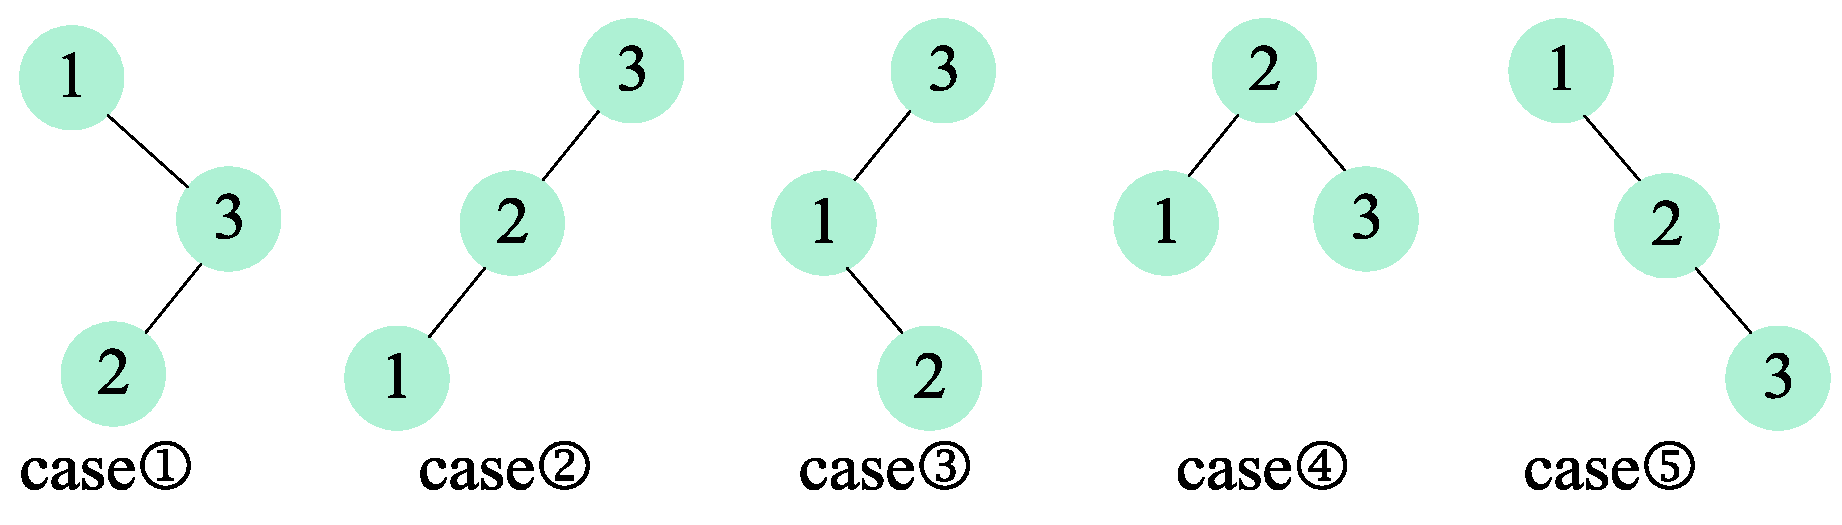
\includegraphics[width=0.7\textwidth]{images/title/二叉搜索树示例.pdf}
		\caption{$n=3$且结构唯一的二叉搜索树示例}
		\label{fig:二叉搜索树示例}
	\end{figure}
    \solution 给定一个有序序列$1\cdots n$, 为了构建出一棵二叉搜索树, 我们可以遍历每个数字 $i$, 将该数字作为根节点, 将$1\cdots i-1$序列作为左子树, 将$i+1,\cdots,n$序列作为右子树. 接着我们可以按照同样的方式递归构建左子树和右子树. 因为根节点的值是彼此互异的, 所以能够保证所构造出的二叉搜索树是不同的(即保证了结构的唯一性). 设$G(n)$是从长度为$n$的序列中所构造出的二叉搜索树的种类数, $F(i,n)$是以$i$($1\leq i\leq n$)为根节点且长度为$n$的序列中构造出的二叉搜索树的种类数\footnote{此题其实跟动态规划没啥本质关系, \textbf{此题本质上就是对计数空间的一个划分(具体体现为$F(i,n)$和$G(n)$的定义差别)}.}. 于是有$$G\left( n \right) =\sum_{i=1}^n{F\left( i,n \right)}
    $$
    接下来计算$F(i,n)$: 从序列$1\cdots i-1$中所构建出的二叉搜索树的个数为$G(i-1)$, 从序列$i+1\cdots n$中所构建出的二叉搜索树的个数为$G(n-i)$. 于是以$i$为根节点的二叉搜索树的种数即为$$F\left( i,n \right) =G\left( i-1 \right) \cdot G\left( n-i \right) 
    $$
    于是题中所求即为$$G\left( n \right) =\sum_{i=1}^n{F\left( i,n \right)}=\sum_{i=1}^n{G\left( i-1 \right) \cdot G\left( n-i \right)}
    $$
    显然$G(0)=1,G(1)=1$, 于是可以写出如下C++代码, 并在\href{https://leetcode.cn/problems/unique-binary-search-trees/description/}{\textbf{LeetCode-T96}}上通过所有测试样例:
\begin{tcblisting}{listing engine=minted,boxrule=0.1mm,
colback=blue!5!white,colframe=blue!75!black,
listing only,left=5mm,enhanced,sharp corners=all,
overlay={\begin{tcbclipinterior}\fill[red!20!blue!20!white] (frame.south west)
rectangle ([xshift=5mm]frame.north west);\end{tcbclipinterior}},
minted language=c++,
minted style=tango,
minted options={fontsize=\small,breaklines,autogobble,linenos,numbersep=3mm}}
class Solution {
public:
    int numTrees(int n) {
        vector<int> G(n + 1, 0);
        G[0] = 1, G[1] = 1;
        for(int i = 2; i <= n; i++) {
            for(int j = 1; j <= i; j++) {
                G[i] += G[j - 1] * G[i - j];
            }
        }
        return G[n];
    }
};
\end{tcblisting}
    \newpage
    其实解答中的$G(n)$就是卡塔兰数, 那么其对应更简单的计算公式为:$$C_0=C_1=1,\quad C_{n+1}=\frac{2\left( 2n+1 \right)}{n+2}C_n
    $$
    于是也可以对应写出C++代码, 并在\href{https://leetcode.cn/problems/unique-binary-search-trees/description/}{\textbf{LeetCode-T96}}上通过所有测试样例:
\begin{tcblisting}{listing engine=minted,boxrule=0.1mm,
colback=blue!5!white,colframe=blue!75!black,
listing only,left=5mm,enhanced,sharp corners=all,
overlay={\begin{tcbclipinterior}\fill[red!20!blue!20!white] (frame.south west)
rectangle ([xshift=5mm]frame.north west);\end{tcbclipinterior}},
minted language=c++,
minted style=tango,
minted options={fontsize=\small,breaklines,autogobble,linenos,numbersep=3mm}}
class Solution {
public:
    int numTrees(int n) {
        vector<long long> C(n + 1, 0);
        C[0] = 1, C[1] = 1;
        for(int i = 1; i < n; i++) {
            C[i + 1] = 2 * (2 * i + 1) * C[i] / (i + 2);
        }
        return (int)C[n];
    }
};
\end{tcblisting}
\end{homeworkProblem}


\begin{homeworkProblem}
    \textbf{回文子串}: 给定字符串$s$, 返回其中回文子串的数目. 注意: 当一个字符串向后读和向前读一样时, 它就是一个回文; 子串是字符串中的\textbf{连续}字符序列.

    \solution \textbf{方法1 (动态规划)}\quad 设$dp[i][j]$表示字符串$s$的字串$s[i\cdots j]$是否为回文串(若为1, 则是回文串; 若为0, 则不是回文串). 若想要判断$s[i\cdots j]$是否回文, 需要以下分类讨论:
    \begin{itemize}
        \item 需先看$s[i],s[j]$: 若$s[i]\neq s[j]$, 那么就肯定不是回文串, 即此时$dp[i][j]=0$; 
        \item 若$s[i]=s[j]$, 那么还需要根据子串$s[i\cdots j]$的长度进一步讨论:
        \begin{itemize}
            \item 如果$i=j$(即子串$s[i\cdots j]$的长度为1), 那么肯定是回文的, 即此时$dp[i][j]=1$;
            \item 如果子串$s[i\cdots j]$的长度为2, 那么肯定也是回文的, 即此时$dp[i][j]=1$;
            \item 如果子串$s[i\cdots j]$的长度$\geq 3$, 因为$s[i]=s[j]$, 所以只需要把两端去掉, 看字串$s[i+1,j-1]$是否为回文串即可, 故而此时$dp\left[ i \right] \left[ j \right] =dp\left[ i+1 \right] \left[ j-1 \right]$.
        \end{itemize}
    \end{itemize}
    综上所述, 该DP算法的转移方程为:
    $$dp\left[ i \right] \left[ j \right] =\begin{cases}
        0, \text{若}s\left[ i \right] \ne s\left[ j \right]\\
        1, \text{若}s\left[ i \right] =s\left[ j \right] \text{且}j-i=0\\
        1, \text{若}s\left[ i \right] =s\left[ j \right] \text{且}j-i=1\\
        dp\left[ i+1 \right] \left[ j-1 \right] , \text{若}s\left[ i \right] =s\left[ j \right] \text{且}j-i\ge 2\\
    \end{cases}
    $$
    合并一下即有:
    $$dp\left[ i \right] \left[ j \right] =\begin{cases}
        0, \text{若}s\left[ i \right] \ne s\left[ j \right]\\
        1, \text{若}s\left[ i \right] =s\left[ j \right] \text{且}j-i<2\\
        dp\left[ i+1 \right] \left[ j-1 \right] , \text{若}s\left[ i \right] =s\left[ j \right] \text{且}j-i\ge 2\\
    \end{cases}
    $$
    其中边界条件为$dp[0][0]=1$. 于是我们可以写出上述算法的C++代码, 并在\href{https://leetcode.cn/problems/palindromic-substrings/description/}{\textbf{LeetCode-T647}}上通过所有测试样例:
\begin{tcblisting}{listing engine=minted,boxrule=0.1mm,
colback=blue!5!white,colframe=blue!75!black,
listing only,left=5mm,enhanced,sharp corners=all,
overlay={\begin{tcbclipinterior}\fill[red!20!blue!20!white] (frame.south west)
rectangle ([xshift=5mm]frame.north west);\end{tcbclipinterior}},
minted language=c++,
minted style=tango,
minted options={fontsize=\small,breaklines,autogobble,linenos,numbersep=3mm}}
class Solution {
public:
    int countSubstrings(string s) {
        int n = s.size(), cnt = 0;
        vector<vector<int>> dp(n, vector<int>(n, 0));
        dp[0][0] = 1;
        for(int j = 0; j < n; j++) {  //注意循环变量i,j的顺序不能反,
            for(int i = 0; i <= j; i++) {  //因为求解方向是从左往右的!
                if(s[i] != s[j]) {
                    dp[i][j] = 0;
                }
                else {
                    if(j - i < 2) {
                        dp[i][j] = 1, cnt++;
                    }
                    else {
                        dp[i][j] = dp[i + 1][j - 1];
                        cnt = cnt + (dp[i][j] == 1 ? 1 : 0);
                    }
                }
            }
        }
        return cnt;
    }
};
\end{tcblisting}
\begin{tcblisting}{listing engine=minted,boxrule=0.1mm,
colback=blue!5!white,colframe=blue!75!black,
listing only,left=5mm,enhanced,sharp corners=all,
overlay={\begin{tcbclipinterior}\fill[red!20!blue!20!white] (frame.south west)
rectangle ([xshift=5mm]frame.north west);\end{tcbclipinterior}},
minted language=c++,
minted style=tango,
minted options={fontsize=\small,breaklines,autogobble,linenos,numbersep=3mm}}
class Solution {
public:
    bool IsPalin(string s) {
        int i = 0, j = s.size() - 1;
        while(i < j) {  //对撞双指针来判断s是否为回文串
            if(s[i] != s[j]) {
                return false;
            }
            else {
                i++, j--;
            }
        }
        return true;
    }
    int countSubstrings(string s) {
        int n = s.size(), cnt = 0;
        for(int i = 0; i < n; i++) {
            for(int j = i; j < n; j++) {
                if(IsPalin(s.substr(i, j - i + 1)) == true) {
                    cnt++;
                }
            }
        }
        return cnt;
    }
};
\end{tcblisting}
    \textbf{方法2 (枚举法)}: 考察所有字串是否为回文串, 算法具体的C++代码如上页中所示, 并在\href{https://leetcode.cn/problems/palindromic-substrings/description/}{\textbf{LeetCode-T647}}上通过所有测试样例. 现在分析一下两个算法的复杂度: 方法1的时空复杂度显然都为$O(n^2)$, 而方法2中有两层for循环, 判断是否为回文串又需要线性的时间, 因此时间复杂度为$O(n^3)$, 空间复杂度显然为$O(1)$. \textbf{借助上面两个算法, 我们还可以求出最长回文子串}, 具体代码如下:
    \\

    \textbf{方法1 (暴力枚举)}: 时间复杂度为$O(n^3)$, 空间复杂度为$O(1)$, 在\href{https://leetcode.cn/problems/longest-palindromic-substring/}{\textbf{LeetCode-T5}}上是超时(但正确)的.
\begin{tcblisting}{listing engine=minted,boxrule=0.1mm,
colback=blue!5!white,colframe=blue!75!black,
listing only,left=5mm,enhanced,sharp corners=all,
overlay={\begin{tcbclipinterior}\fill[red!20!blue!20!white] (frame.south west)
rectangle ([xshift=5mm]frame.north west);\end{tcbclipinterior}},
minted language=c++,
minted style=tango,
minted options={fontsize=\small,breaklines,autogobble,linenos,numbersep=3mm}}
class Solution {
public:
    bool IsPalindrome(string s) {
        int i = 0, j = s.size() - 1;
        while(i < j) {
            if(s[i] != s[j]) {
                return false;
            }
            else {
                i++, j--;
            }
        }
        return true;
    }
    string longestPalindrome(string s) {
        int n = s.size(), L = 1, index = 0;
        string res;
        if(n < 2) res = s;
        for(int i = 0; i < n; i++) {
            for(int j = i; j < n; j++) {
                if(IsPalindrome(s.substr(i, j - i + 1)) == true) {
                    if(j - i + 1 > L) {
                        L = j - i + 1;
                        index = i;
                    }
                }
            }
        }
        return s.substr(index, L);
    }
};
\end{tcblisting}
    \newpage
    \vspace{2cm}
    \textbf{方法2 (动态规划)}: 时间复杂度为$O(n^2)$, 空间复杂度也为$O(n^2)$, 在\href{https://leetcode.cn/problems/longest-palindromic-substring/}{\textbf{LeetCode-T5}}上通过所有测试样例:
\begin{tcblisting}{listing engine=minted,boxrule=0.1mm,
colback=blue!5!white,colframe=blue!75!black,
listing only,left=5mm,enhanced,sharp corners=all,
overlay={\begin{tcbclipinterior}\fill[red!20!blue!20!white] (frame.south west)
rectangle ([xshift=5mm]frame.north west);\end{tcbclipinterior}},
minted language=c++,
minted style=tango,
minted options={fontsize=\small,breaklines,autogobble,linenos,numbersep=3mm}}
class Solution {
public:
    string longestPalindrome(string s) {
        int n = s.size(), L = 1, index = 0;
        string res;
        if(n < 2) res = s;
        vector<vector<int>> dp(n, vector<int>(n, 0));
        dp[0][0] = 1;
        for(int j = 0; j < n; j++) {  //注意循环变量i,j的顺序不能反,
            for(int i = 0; i <= j; i++) {  //因为求解方向是从左往右的!
                if(s[i] != s[j]) {
                    dp[i][j] = 0;
                }
                else {
                    if(j - i < 2) {
                        dp[i][j] = 1;
                        if(L < j - i + 1) {
                            L = j - i + 1;
                            index = i;
                        }
                    }
                    else {
                        dp[i][j] = dp[i + 1][j - 1];
                        if(dp[i][j] == 1) {
                            if(L < j - i + 1) {
                                L = j - i + 1;
                                index = i;
                            }
                        }
                    }
                }
            }
        }
        return s.substr(index, L);
    }
};
\end{tcblisting}
    至此, Chap 3所有作业题目都已解答完毕.
\end{homeworkProblem}



% 引用文献
\bibliographystyle{unsrt}  % unsrt:根据引用顺序编号
\bibliography{refs}


\end{document}
